\documentclass[12pt, letterpaper, twoside]{article}
\usepackage[utf8]{inputenc}

\usepackage{xcolor}
\usepackage{sectsty}
\sectionfont{\color{blue}}  
\subsectionfont{\color{cyan}}  

\usepackage{graphicx}

\title{\color{cyan}IKEcoin: \\ 
\large A decentralized authentication protocol and token economy empowering humans to own and sell their own social media data}
\author{Claire Longo, Isaac Longo}
\date{June 2021}

\begin{document}

\maketitle

\begin{figure}[h]
  
\includegraphics[scale=0.5]{media/IKEcoin.jpg}
  \centering
\end{figure}

\begin{abstract}
  \noindent
  beep boop bop
\end{abstract}


\section{Motivation}
blah blah blah

\section{System Design}
blah blah blah


\section{Token Economics}
blah blah blah


\section{User-Customer Transacton example}
\subsubsection*{Economic Agents}
\begin{itemize}
\item \textit{User}\textbf{---}An individual consumer who has established ownership over their data by claiming their IKEcoin and connecting their social media accounts to their token.
\item \textit{Customer}\textbf{---}A company seeking to obtain access and legal authorization to the User's data.
\end{itemize}

There are several steps in a successful IKEcoin transaction between the User and Customer. Consider this example where Isaac is an avid social media user with a passion for skiing, and he is connecting his data with an e-commerce company specialized in selling ski equipment. The steps in the transaction are;
\begin{enumerate}

\item Isaac sets up his IKEcoin account by claiming his IKEcoin at ikecoin.com. He connects his social media accounts to his IKEcoin auth protocol.
\begin{figure}[h]
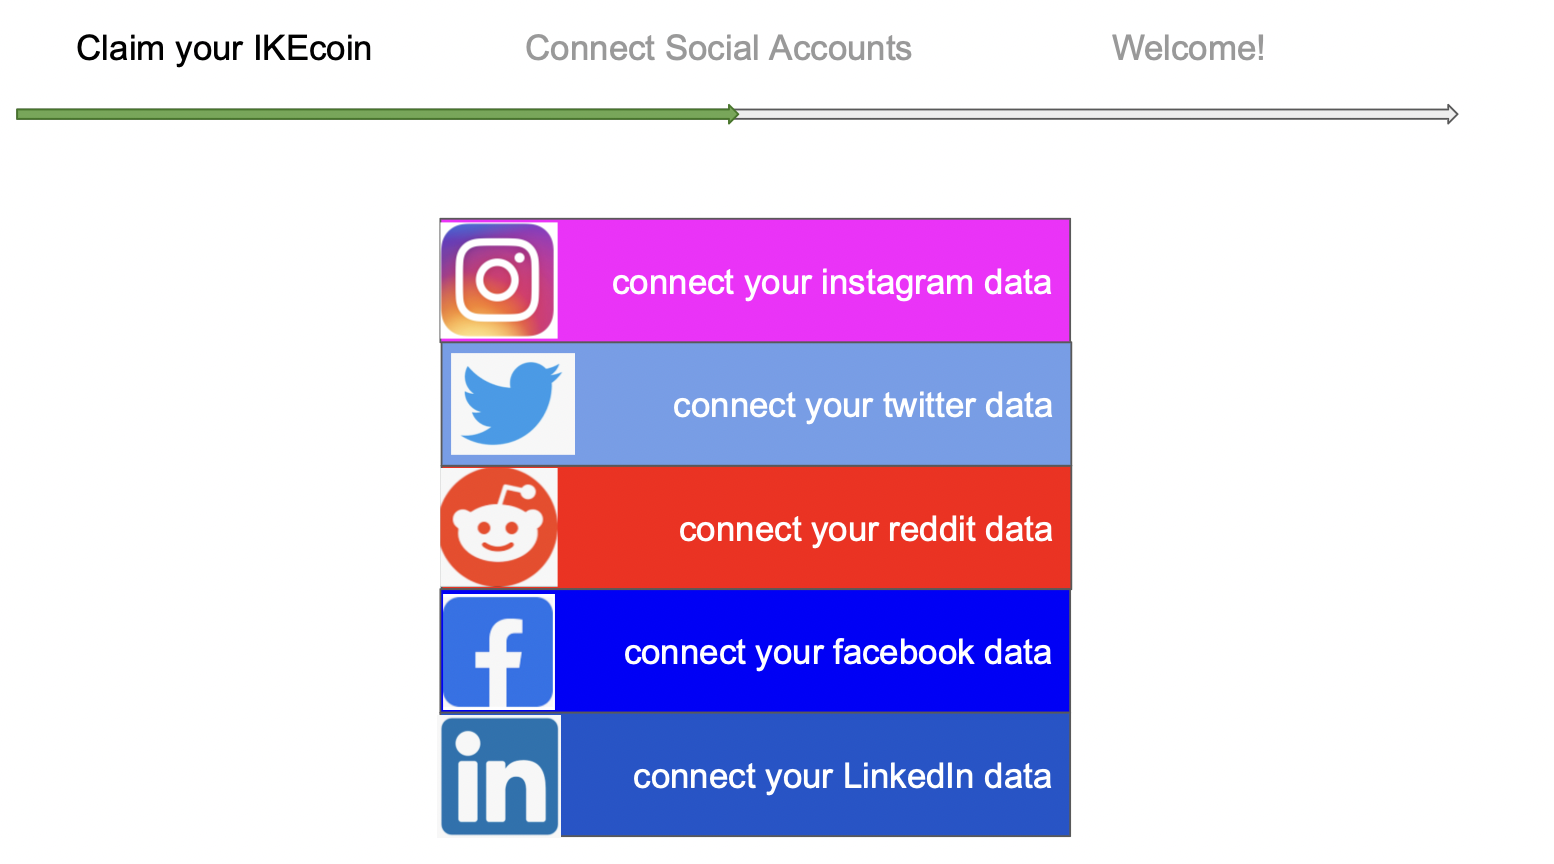
\includegraphics[scale=0.3]{media/AddSocial.jpg}
\centering
\end{figure}
  
\item The value of his IKEcoin is based on the fair market value for the data, the number of accounts linked, and the size of the data he connected
\begin{figure}[h]
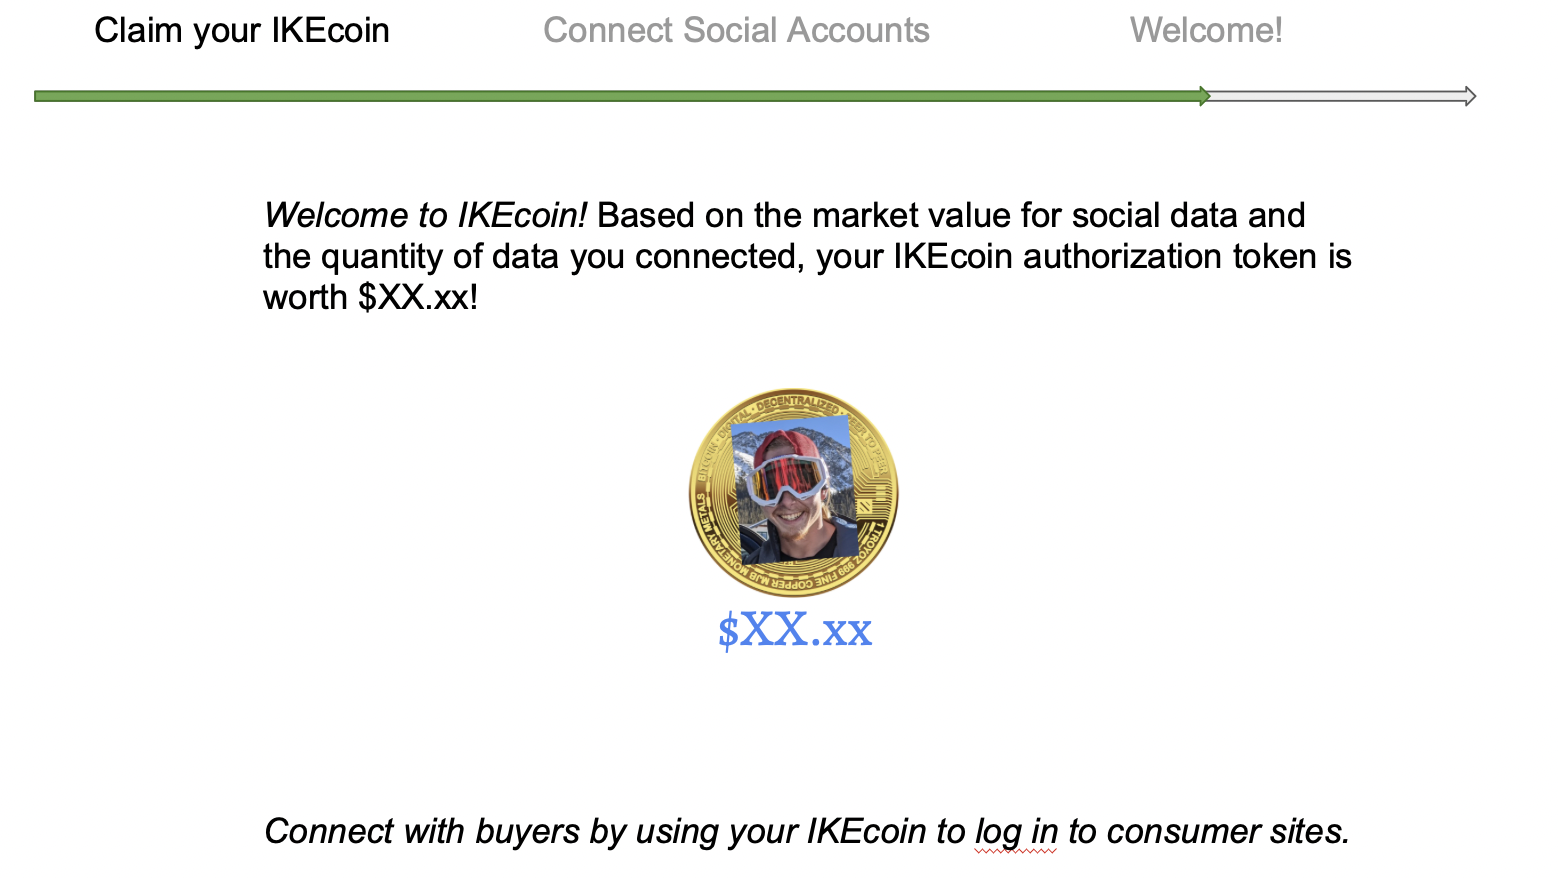
\includegraphics[scale=0.3]{media/Welcome.jpg}
\centering
\end{figure}
   
\item An e-commerce company focused on selling ski equipment has enabled IKEcoin auth at login. They have written a clear terms of service agreement detailing how they will use data obtained through IKEcoin auth. Isaac accepts this agreement and uses his IKEcoin auth to log in to the website 
\begin{figure}[h]
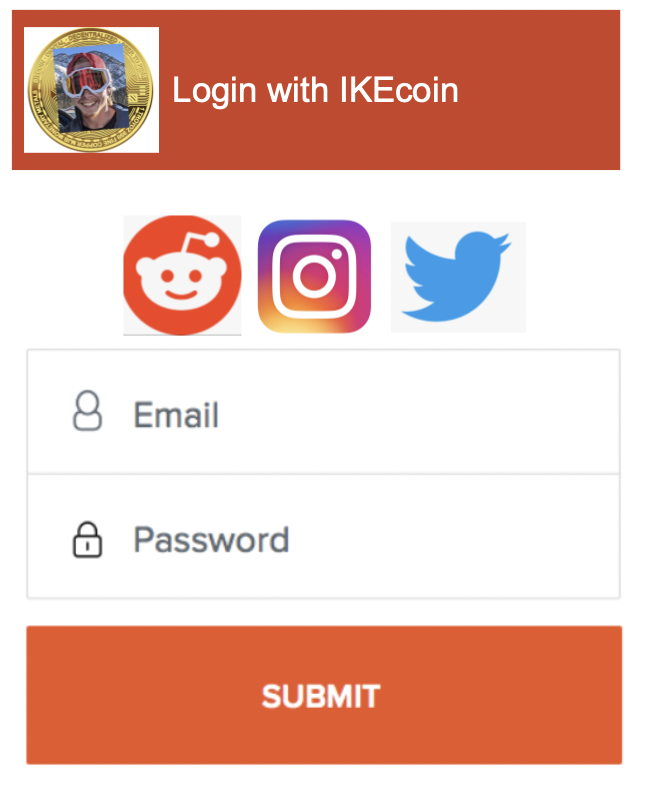
\includegraphics[scale=0.3]{media/IKEcoinLogin.jpg}
\centering
\end{figure}
    
\item The e-commerce site pays Isaac for access to his data  in IKEtokens
    
\item The e-commerce website uses Isaac's social media data to improve their ML algorithm that gives personalized product recommendations 
    
\item Isaac buys the new set of ski boots recommended to him by the ML algorithm    
\end{enumerate}

\subsubsection*{Benefit to the User}
\begin{itemize}
\item The User is able to directly profit from the sale of their data
\item The User can choose who to sell their data to
\end{itemize}


\subsubsection*{Benefit to the Customer}
\begin{itemize}
\item Customer can easily collect large amounts of data on their users
\item The customer can obtained direct legal authorization from the User to access and use their data
\item The data for a single user is already joined across multiple social accounts so they can create a coherent user journey and easily manage their customer's profiles
\end{itemize}



\section{Roadmap/MVP definition}
blah blah blah

\section{Conclusion}
blah blah blah

\end{document}